%%%%%%%%%
\section{Thursday 30 August:  Scan Conversion of a Triangle}
%%%%%%%%%%%

\subsection{Homework 1} due 13 September

{\it Callback}  Do sth when sth happens

Will have global variables

Assignment is given as a triangle with a certain order of $x_0$, $x_1$, and $x_2$.  Extra part of assignment is to account for different orders.  

\

\subsection{Midpoint Algorithm (Besenham) Pseudocode}

Initialize integers $\Delta_E$, $\Delta_{NE}$, $d$, $x$, and $y$.  

Set pixel at $(x,y)$ (first pixel)

\

{\bf while} $x$ $<$ last column (given by an endpoint)

\{

	\qquad increment $x$ by 1
	
	\qquad {\bf if} ($d<0$)
	
		\qquad \qquad add $\Delta _E$ to $d$
	
	\qquad {\bf else}
	
	\qquad \{
	
		\qquad \qquad increment $y$ by 1
		
		\qquad \qquad add $\Delta_{NE}$ to $d$
	
	\qquad \}
	
	\qquad set pixel at $(x,y)$

\}

\

\subsection{Naming Conventions}

\hfil\begin{tikzpicture}[x=16mm, y=16mm]
	\coordinate (A) at (0,0);
	\coordinate (B) at (-4,4);
	\coordinate (C) at (2,6);
	\draw (A) -- (B) -- (C) -- (A);
	\path (A) node [below] {$(x_0,y_0,R_0,G_0,B_0)$};
	\path (B) node [left] {$(x_1,y_1,R_1,G_1,B_1)$};
	\path (C) node [above] {$(x_2,y_2,R_2,G_2,B_2)$};
	
	\coordinate (M01) at (-2,2);
	\coordinate (L01) at ($(M01) - ({1/sqrt(2)},{1/sqrt(2)})$);
	\node (NM01) at (M01) {};
	\node (NL01) at (L01) {$L_{0,1}$};
	\draw [->] (NL01) -- (NM01);

	\coordinate (M02) at (1,3);
	\coordinate (L02) at ($(M02) + ({3/sqrt(10)},{-1/sqrt(10)})$);
	\node (NM02) at (M02) {};
	\node (NL02) at (L02) {$L_{0,2}$};
	\draw [->] (NL02) -- (NM02);

	\coordinate (M12) at (-1,5);
	\coordinate (L12) at ($(M12) + ({-1/sqrt(10)},{3/sqrt(10)})$);
	\node (NM12) at (M12) {};
	\node (NL12) at (L12) {$L_{1,2}$};
	\draw [->] (NL12) -- (NM12);

\end{tikzpicture}

Simplifying Assumptions:

\qquad Vertices have integer coordinates

\qquad $y_0 \le y_1 \le y_2$

\

{\bf Idea}

We want to interpolate the colors to get shading.  

Look at the triangle one scan line at a time, looping bottom to top, left to right.  

\

Two loops

\qquad One for the bottom

\qquad One for the top

\

\hfil\begin{tikzpicture}[x=8mm, y=8mm]
	\coordinate (V0) at (0,0);
	\coordinate (V1) at (-4,4);
	\coordinate (V2) at (2,6);
	\draw (V0) -- (V1) -- (V2) -- (V0);
	\path (V0) node [below] {$(x_0,y_0,R_0,G_0,B_0)$};
	\path (V1) node [left] {$(x_1,y_1,R_1,G_1,B_1)$};
	\path (V2) node [above] {$(x_2,y_2,R_2,G_2,B_2)$};
	
	\coordinate (M01) at ($(V0)!0.5!(V1)$);
	\coordinate (L01) at ($(M01) - ({1/sqrt(2)},{1/sqrt(2)})$);
	\node (NM01) at (M01) {};
	\node (NL01) at (L01) {$L_{0,1}$};
	\draw [->] (NL01) -- (NM01);

	\coordinate (M02) at ($(V0)!0.5!(V2)$);
	\coordinate (L02) at ($(M02) + ({3/sqrt(10)},{-1/sqrt(10)})$);
	\node (NM02) at (M02) {};
	\node (NL02) at (L02) {$L_{0,2}$};
	\draw [->] (NL02) -- (NM02);

	\coordinate (M12) at ($(V1)!0.5!(V2)$);
	\coordinate (L12) at ($(M12) + ({-1/sqrt(10)},{3/sqrt(10)})$);
	\node (NM12) at (M12) {};
	\node (NL12) at (L12) {$L_{1,2}$};
	\draw [->] (NL12) -- (NM12);
	
	\draw [dashed] (V1) -- ({4/3},4);
	
\end{tikzpicture}

\

{\bf Scan Line}

\

\hfil\begin{tikzpicture}[x=16mm, y=16mm]
	\coordinate (V0) at (0,0);
	\coordinate (V1) at (-4,4);
	\coordinate (V2) at (2,6);
	\draw (V0) -- (V1) -- (V2) -- (V0);
	\path (V0) node [below] {$(x_0,y_0,R_0,G_0,B_0)$};
	\path (V1) node [left] {$(x_1,y_1,R_1,G_1,B_1)$};
	\path (V2) node [above] {$(x_2,y_2,R_2,G_2,B_2)$};
	
	\coordinate (M01) at ($(V0)!0.8!(V1)$);
	\coordinate (L01) at ($(M01) - ({1/sqrt(2)},{1/sqrt(2)})$);
	\node (NM01) at (M01) {};
	\node (NL01) at (L01) {$L_{0,1}$};
	\draw [->] (NL01) -- (NM01);

	\coordinate (M02) at ($(V0)!0.8!(V2)$);
	\coordinate (L02) at ($(M02) + ({3/sqrt(10)},{-1/sqrt(10)})$);
	\node (NM02) at (M02) {};
	\node (NL02) at (L02) {$L_{0,2}$};
	\draw [->] (NL02) -- (NM02);

	\coordinate (M12) at ($(V1)!0.5!(V2)$);
	\coordinate (L12) at ($(M12) + ({-1/sqrt(10)},{3/sqrt(10)})$);
	\node (NM12) at (M12) {};
	\node (NL12) at (L12) {$L_{1,2}$};
	\draw [->] (NL12) -- (NM12);
	
	\draw [dashed] (V1) -- ({4/3},4);
	
	\coordinate (sL) at (-3,1.5);
	\coordinate (sR) at (2,1.5);
	\draw [dashed] (sL) -- (sR) node [right] {Scan line};
	
	\coordinate (xL) at (intersection of V0--V1 and sL--sR);
	\coordinate (xR) at (intersection of V0--V2 and sL--sR);
	\fill (xL) circle (5pt) node [below left] {$(x_L,y)$};
	\fill (xR) circle (5pt) node [below right] {$(x_R,y)$};

\end{tikzpicture}

\subsection{Line Scan Pseudocode}

for $y$ from $y_0$ to $(y_1 - 1)$

\{

\qquad Calculate coordinates where scan line intersects $L_{0,1}$ and $L_{0,2}$.  

\qquad \qquad ({\it i.e.} Calculate $x_L$ and $x_R$ incrementally)

\qquad Color the pixels from $\left( \lceil x_L \rceil, y \right)$ to $\left( \lfloor x_R \rfloor, y \right)$


\}



\

for $y$ from $y_1$ to $y_2$

\{

\qquad Calculate coordinates where scan line intersects $L_{1,2}$ and $L_{0,2}$.  

\qquad \qquad ({\it i.e.} Calculate $x_L$ and $x_R$ incrementally)

\qquad Color the pixels from $\left( \lceil x_L \rceil, y \right)$ to $\left( \lfloor x_R \rfloor, y \right)$


\}

\subsection{Special Cases}

{\bf Watch for division by zero!}

Horizontal lines, either between $V_0$ and $V_1$ or between $V_1$ and $V_2$.  

\subsection{Calculating $x_L$ and $x_R$ Incrementally}

\begin{tabular}{p{4in}p{2in}}

Initialize $x_L = x_0$, $x_R = x_0$, $y = y_0$

Note that $y$ is being incremented by 1.  
\

$\displaystyle x_{i+1} = x_i + \frac{1}{m} = x_i + \frac{x_1 - x_0}{y_1 - y_0}$

\

$\displaystyle x_L = x_L +  + \frac{x_1 - x_0}{y_1 - y_0}$

\

$\displaystyle x_R = x_R +  + \frac{x_2 - x_0}{y_2 - y_0}$

&
\hfill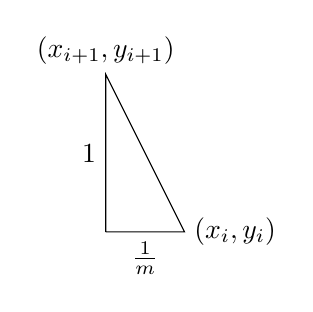
\begin{tikzpicture}[baseline=(current bounding box.north),x=10mm, y=10mm]
	\coordinate (A) at (0,0);
	\coordinate (B) at (1,0);
	\coordinate (C) at (0,2);
	\draw (A) -- (B) -- (C) -- (A);
	\path (B) node [right] {$(x_i,y_i)$};
	\path (C) node [above] {$(x_{i+1}, y_{i+1})$};
	\path (A) -- (B) node [midway, below] {$\frac{1}{m}$};
	\path (A) -- (C) node [midway, left] {1};
\end{tikzpicture}

\cr
\end{tabular}

\subsection{Color}

{\color{red}
	Notes on this section:  
	
	Make sure we're consistent about when to use $x_L - x_R$ and when to use $\lceil x_L \rceil - \lfloor x_R \rfloor$.
}

\

Computing color incrementally (Here considering only R, red)

Initialize $R_L = R_0$, $R_R = R_0$

For each scan line:

\

\qquad $\displaystyle R_L = R_L + \frac{R_1 - R_0}{y_1 - y_0}$

\

\qquad $\displaystyle R_R = R_R + \frac{R_2 - R_0}{y_2 - y_0}$

\

Within a scan line, between $\lceil x_L \rceil$ and $\lfloor  x_R \rfloor$

\

\qquad Initialize $\displaystyle R = R_L + \frac{R_L - R_R}{x_L - x_R} \left( \lceil x_L \rceil - x_L \right)$

\qquad Color first pixel

\qquad for $R$ from $R_L$ to $R_R$

\qquad \{

\qquad \qquad $\displaystyle R = R + \frac{R_L - R_R}{\lceil x_L \rceil - \lfloor x_R \rfloor } $

\qquad \qquad [Do the same for $G$ and $B$.]

\qquad \qquad Color pixel $(x, y, R, G, B)$

\qquad \}

